%%%%%
% multiline comment
%%%%%

% single line comment

\documentclass[12pt, letterpaper]{article}
% set custom margins
\usepackage[a4paper, left=.75in, top=.75in, bottom=0.75in]{geometry}

% remove indents from paragraphs
\setlength{\parindent}{0pt}


% PACKAGES USED IN THIS DOCUMENT 

% allow for images to be added, specify folder path between second pair of curly braces
\usepackage{graphicx}
\graphicspath{ {./images/} }

% PACKAGES USED IN THIS DOCUMENT 
% allow for multiple columns
\usepackage{multicol}

% math-related packages
\usepackage{mathtools} 
\usepackage{amssymb}
\usepackage{amsmath}

% create links in document
\usepackage{hyperref}

% create graphs and charts 
\usepackage{tikz}
\usetikzlibrary{automata, positioning}

% change spacing to share title page with content
\title{\vspace{-15pt}title}
\author{author}
%change spacing for date to be closer to name
\date{\vspace{-3pt}date}

\begin{document}
\maketitle

\section{Create Section Heading}
\subsection{create smaller sub-section heading}

\textbf{Bold Text!} normal text

\emph{italicized text} normal text

% numbered list
\begin{enumerate}
    \item 
    
    \item  
    
    \item  

    \item 

    \item 
    
\end{enumerate}

% create a line break 10pts tall
\vskip 10pt

\subsection{create a multi-column layout}
In the instance below, it's only two columns. 
% create a two-column layout, specified as two with {2}, could be more
\begin{multicols}{2}

Text goes here for column 1. 

\columnbreak

Text goes here for column 2. 

\end{multicols}

\vskip 10pt
\subsection{create a multi-column table}
% create a centered two-column table with lines for each row
\begin{center}
% adding more " |c| " will add more columns to the table 
\begin{tabular}{ |c|c| }
\hline
Column 1 Heading & Column 2 Heading \\
% h-line adds the lines between rows
\hline
% the " & " specifies to start the next column
Column 1 & Column 2 \\
\hline
Column 1 & Column 2 \\
\hline
Column 1 & Column 2 \\
\hline
Column 1 & Column 2 \\
\hline
\end{tabular}
\end{center}

\subsection{include images}
You'll need to specify a folder path in the document metadata, as well as the folder and image name in the curly braces.
% include a centered image
\begin{center}
% set scale of image to 60% of full size
\includegraphics[scale=0.6]{images-folder/image-name.png}
\end{center}

\subsection{useful theory of computation syntax:}
% useful Theory of Computation syntax: 
Formal Definition:
M = $\{ Q, \Sigma, q, \delta, F \}$
$ \forall $
$ \in $
$ \exists $
% capitalizing greek names for letters will make the letter uppercase
$ \Sigma $ 
$ \sigma $ 
$ \epsilon $
$ \rightarrow $

%greater than equal to
$ \geq $

%greater than
% \gt 

% not equal
$ \neq $

%arrow pointing both ways
$ \leftrightarrow $ 

$ \subseteq $

PART THREE: Design A Deterministic Finite Automaton

Assume the alphabet $( \Sigma = \{0, 1\} )$ and \emph{L} = \{100\} $\subset \Sigma^*$ . Please design a DFA whose language is \emph{L}.

% Formal Definition:
% M = \{ Q, \Sigma, q, \delta, F \}
% \forall
% \in
% \exists
% $\epsilon$

\begin{center}
    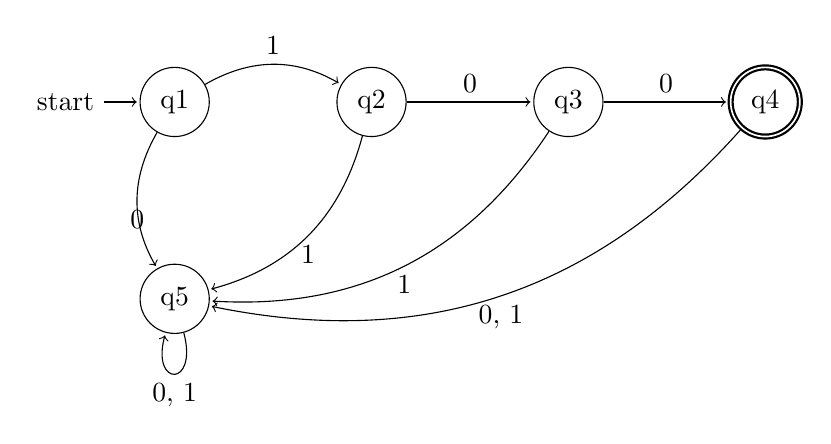
\begin{tikzpicture}[shorten >=1pt, node distance=2.5cm, on grid, auto]
        % define states
        % initial state
        \node[state, initial] (q1)   {q1}; 
        \node[state] (q2) [right=of q1] {q2}; 
        \node[state] (q3) [right=of q2] {q3};
        % q4 accept state
        \node[state, accepting, thick] (q4) [right=of q3] {q4}; 
        % q5 is below q1
        \node[state] (q5) [below=of q1] {q5}; 

        % define transitions
        \path[->]
        % q1 to q2 if input = 1
        (q1) edge [bend left, above] node {1} (q2) 
            % q1 to q5 if input = 0
              edge [bend right, below] node {0} (q5) 
        (q2) edge node {0} (q3) % q2 to q3 if input = 0
            edge [bend left, below] node {1} (q5) % q2 to q5 if input = 1
        (q3) edge node {0} (q4) % q3 to q4 if input = 0; accept state for 100
            edge [bend left, below] node {1} (q5) % q3 to q5 if input = 1
        (q4) edge [bend left, below] node {0, 1} (q5) % q4 to q5 if additional inputs
        % q5 loop back to q5 if input = 0 or 1
        (q5) edge [loop below] node {0, 1} (q5); 
    \end{tikzpicture}
\end{center}

% example Turing Machine Syntax:
$ q \square\$ \rightarrow qN \$ $

$ q_1 \square\$ \rightarrow q_1 N\$ $

$ q_1 \square1 \rightarrow q_1 N1 $

$ q_3 0 \rightarrow q_{reject} $

$ q_3\square \rightarrow q_{accept} $

\subsection{useful probability and statistics syntax:}
% useful Probability and Statistics syntax

\textbf{3 - Test Statistic}
\vskip 12pt

\begin{center}
$ \mathbf{t = \frac{\bar{x}_1 - \bar{x}_2}{\sqrt{(\frac{(s_1)^2}{n_1}) + (\frac{(s_2)^2}{n_2})}} }$
\end{center}


First, finding $ \mathbf{\frac{(s_1)^2}{n_1}} $ and $ \mathbf{\frac{(s_2)^2}{n_2}} $ to use later when calculating $ \mathbf{\nu} $.
\vskip 9pt
$ ((s_1)^2/n_1) = (33.27^2)/25 \approx 44.2757 $
\vskip 9pt
$ ((s_2)^2/n_2) = (47.92^2)/25 \approx 91.8531 $
\vskip 9pt
$ t = (143.28 - 211.56)/\sqrt{(44.2757 + 91.8531)} $
\vskip 9pt
$ t = (-68.28)/\sqrt{136.1288} $
\vskip 9pt
$ t \approx -5.85 $

\vskip 12pt
\textbf{4A - Rejection Region}

\begin{center}
$ \mathbf{\nu = \frac{((s_1)^2/n_1)-(s_2)^2/n_2))^2}{(\frac{(((s_1)^2)/n_1)^2}{n_1-1})+(\frac{(((s_2)^2)/n_2)^2}{n_2-1})}} $
\end{center}
$ t_{\alpha,\nu} = t_{0.05, \nu} $
\vskip 9pt
$ \nu = \frac{(44.2757+91.8531)^2}{(\frac{44.2757^2}{25-1})+(\frac{91.8531^2}{25-1})} $
\vskip 9pt
$ \nu = \frac{(136.1288)^2}{(\frac{1960.3376}{24})+(\frac{8436.9920}{24})} $
\vskip 9pt
$ \nu = \frac{18531.0502}{(81.6807)+(351.5413)} $
\vskip 9pt
$ \nu = \frac{18531.0502}{433.222} $
\vskip 9pt
$ \nu \approx 42.77 \approx 43 $

\vskip 12pt
$ t_{0.05, 43} \approx 1.681 $

\vskip 12pt
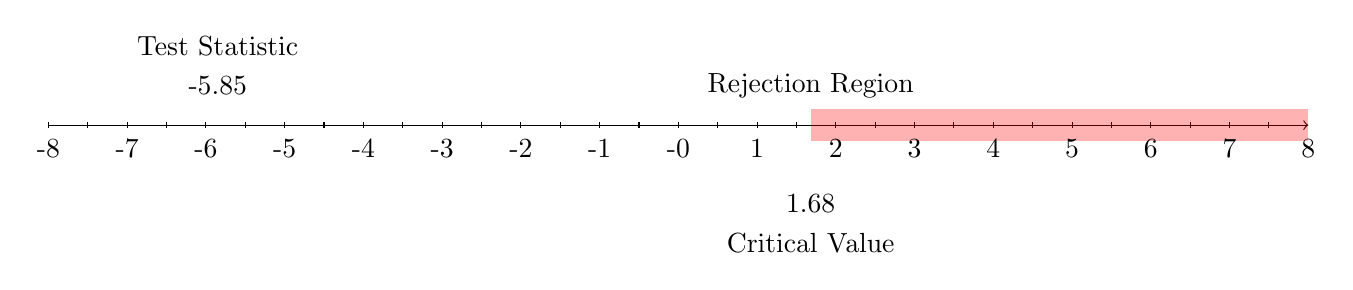
\begin{tikzpicture}
    % Draw number line
    \draw[->] (-8,0) -- (8,0); 
    \foreach \x in {-8, -7.5, -7, -6.5, -6, -5.5, -5, -4.5, -4, -3.5, -3, -2.5, -2, -1.5, -1, -0.5, 0, 0.5, 1, 1.5, 2, 2.5, 3, 3.5, 4, 4.5, 5, 5.5, 6, 6.5, 7, 7.5} % Tick marks
        \draw[shift={(\x,0)}] (0,1pt) -- (0,-1pt);

    % Label the number line
    \node at (-5.85, 1) {Test Statistic};

    % Rejection region shading
    \fill[red, opacity=0.3] (1.68, -0.2) rectangle (8, 0.2);

    % Critical value
    \node at (1.681, -1.5) {Critical Value};

    % Rejection region
    \node at (1.68, 0.5) {Rejection Region};

    % Add numerical labels at specific points
    \node at (-8, -0.3) {-8};
    \node at (-7, -0.3) {-7};
    \node at (-6, -0.3) {-6};
    \node at (-5.85, 0.5) {-5.85};
    \node at (-5, -0.3) {-5};
    \node at (-4, -0.3) {-4};
    \node at (-3, -0.3) {-3};
    \node at (-2, -0.3) {-2};
    \node at (-1, -0.3) {-1};
    \node at (0, -0.3) {-0};
    \node at (1, -0.3) {1};
    \node at (1.68, -1) {1.68};
    \node at (2, -0.3) {2};
    \node at (3, -0.3) {3};
    \node at (4, -0.3) {4};
    \node at (5, -0.3) {5};
    \node at (6, -0.3) {6};
    \node at (7, -0.3) {7};
    \node at (8, -0.3) {8};
\end{tikzpicture}

The test statistic is not within the rejection region. 

\end{document}
